% !TEX root = index.tex

\section{Vector spaces}

\subsection{Motivation}
\label{section:VectorSpaces}
A \emph{scalar} is a real number.
A (column) \emph{vector} $\vec{v}$ of size $n$ is a column of $n$ scalars
\begin{align*}
  \vec{v} =
  \begin{bmatrix}
    v_1 \\
    v_2 \\
    \vdots \\
    v_n
  \end{bmatrix}
\end{align*}
The scalars $v_i$ are called the \textit{coordinates} of $\vec{v}$.
The set of all (column) vectors is called the \emph{Euclidean space} of dimension $n$ and is denoted by $\bbr^n$.
Denote by $\vec{0}$ the vector with all coordinates 0.
$\vec{e}_i$ is the vector whose $i^{th}$ coordinate is 1 and all other coordinates are 0.
The vector $\vec{e}_i$ is called the \emph{$i^{th}$ standard basis vector} and the collection $\calb= \set{\vec{e}_1, \dots, \vec{e}_n}$ is called the \emph{standard basis}.

The spaces $\bbr^1$, $\bbr^2$, $\bbr^3$ are very commonly studied objects, but unfortunately, most of us are unable to visualize the higher dimensions.
Linear algebra is the language that lets us do exactly this.

\begin{figure}[H]
  \centering
  \begin{subfigure}[b]{0.45\textwidth}
    \begin{tikzpicture}
  \draw [dashed] (0,1)--(5,1) node [below] {$\bbr^1$};
  \node at (5,-0.25) {$ $};
  \draw [fill] (2,1) circle [radius=0.05] node [above left] {$\vec{0} = [0]$};
  \draw [fill] (3.5,1) circle [radius=0.02] node [above right] {$[1]$};
  \draw [->, thick] (2,1)--(3.5,1);
\end{tikzpicture}

    \caption*{$\bbr^1$ is the real line,}
  \end{subfigure}
  \hfill
  \begin{subfigure}[b]{0.45\textwidth}
    \begin{tikzpicture}
  \draw [dashed] (0,0)--(3.5,0);
  \draw [dashed] (1.5,-1)--(1.5,2.5);
  \draw [->, thick] (1.5,0)--(1.5,1.5);
  \draw [fill] (1.5,0) circle [radius=0.05]
    node [below left] {$\vec{0} = \begin{bmatrix} 0 \\ 0 \end{bmatrix}$};
  \draw [fill] (3,0) circle [radius=0.02]
    node [above right] {$\vec{e}_1 = \begin{bmatrix} 1 \\ 0 \end{bmatrix}$};
    \draw [fill] (1.5,1.5) circle [radius=0.02]
      node [left] {$\vec{e}_2 = \begin{bmatrix} 0 \\ 1 \end{bmatrix}$};
  \node [below] at (5,0) {$\bbr^2$};
  \draw [->, thick] (1.5,0)--(3,0);
  \draw [->, thick] (1.5,0)--(3,3);
    \node [below right] at (3,3) {$\begin{bmatrix} 1 \\ 2 \end{bmatrix}$};
\end{tikzpicture}

    \caption*{$\bbr^2$ is the Euclidean plane,}
  \end{subfigure}
\end{figure}
\begin{figure}[H]
  \centering
  \begin{subfigure}[b]{0.45\textwidth}
    \tdplotsetmaincoords{105}{-30}
\begin{tikzpicture}[tdplot_main_coords,font=\sffamily,scale=0.7]
 \tdplotsetrotatedcoords{00}{30}{0}
 \begin{scope}[tdplot_rotated_coords]
  \begin{scope}[canvas is xy plane at z=0]
   \fill[gray,fill opacity=0.3] (-2,-3) rectangle (2,3);
   \path (-150:2) coordinate (H) (-1.5,0) coordinate(X);
   \pgflowlevelsynccm
  \end{scope}
  \draw[very thick,-stealth] (0,0,0) coordinate (O) -- (0,0,3) node[right]{$\vec{v}$};
 \end{scope}
 \pgfmathsetmacro{\Radius}{1.5}
 \draw[-stealth]  (O)-- (2.5*\Radius,0,0) node[pos=1.15] {$y$-axis};
 \draw[-stealth] (O) -- (0,3.5*\Radius,0) node[pos=1.15] {$x$-axis};
 \draw[-stealth] (O) -- (0,0,2.5*\Radius) node[pos=1.05] {$z$-axis};
\end{tikzpicture}

    \caption*{$\bbr^3$ is the three dimensional space,}
  \end{subfigure}
  \hfill
  \begin{subfigure}[b]{0.45\textwidth}
    {\Huge \begin{align*}
      ?
    \end{align*}}
    \caption*{What does $\bbr^n$ look like?}
  \end{subfigure}
\end{figure}


There are two operations we can perform on vectors in $\bbr^n$:
\begin{enumerate}
  \item\textbf{Scalar multiplication:} Given a scalar $c$ and a vector $\vec{v}$, the vector $c \vec{v}$ is the vector obtained by multiplying every coordinate of $\vec{v}$ by $c$.

  Geometrically, this is scaling the vector $\vec{v}$ by a factor of $c$.\footnote{If $c$ is negative, we ``flip'' $\vec{v}$ across the origin.}

  \item\textbf{Addition:} Given two vectors $\vec{v}$, $\vec{w}$, the sum $\vec{v} + \vec{w}$ is the vector obtained by adding the respective coordinates.

  Geometrically, vector addition is given by the Parallelogram Law.
\end{enumerate}
\begin{qbox}
  \label{q:parallelogramLaw}
    Let $\vec{v} = \begin{bmatrix}v_1 \\ v_2\end{bmatrix}$ and $\vec{w} = \begin{bmatrix}w_1 \\ w_2\end{bmatrix}$ be vectors in $\bbr^2$.
    Verify that
    \begin{align*}
      \vec{0}, \: \vec{v}, \: \vec{v} + \vec{w}, \: \vec{w}
    \end{align*}
    form the vertices of a parallelogram.\tablefootnote{Here we are thinking of vectors as points. It can be a bit confusing at first, to switch between points and arrows, but this flexibility is very useful once you get used to it.}
    This is called the \textit{parallelogram law of vector addition}. The parallelogram law holds even for $\bbr^n$.
    \begin{figure}[H]
      \centering
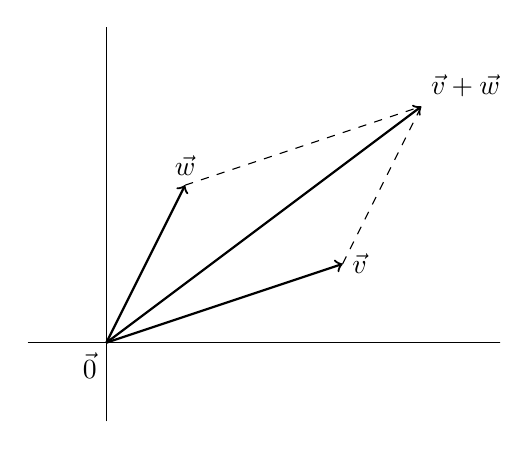
\begin{tikzpicture}
  \clip(-1,-1) rectangle (5,4);
  \draw (0,-1)--(0,10);
  \draw (-1,0)--(10,0);

  \draw [thick, ->] (0,0)--(3,1);
  \node [below left] at (0,0) {$\vec{0}$};
    \node [right] at (3,1) {$\vec{v}$};
  \draw [thick, ->] (0,0)--(1,2);
    \node [above] at (1,2) {$\vec{w}$};
  \draw [dashed] (1,2)--(4,3);
  \draw [dashed] (3,1)--(4,3);
  \draw [thick, ->] (0,0)--(4,3);
    \node [above right] at (4,3) {$\vec{v} + \vec{w}$};
\end{tikzpicture}

      \caption{Parallelogram law of vector addition.}
    \end{figure}
\end{qbox}










\subsubsection{Lines and planes in $\bbr^3$}
A line in $\bbr^2$ is given by an equation $y = mx + c$. What about a line in $\bbr^3$?
One way to decribe a line in $\bbr^3$ is using vector notation.
\begin{ex}
  \label{example:lineAsSpan}
  Every line $L$ in $\bbr^3$ passing through the origin can be written as
  \begin{align*}
    L = \set{c \vec{v} : c \in \bbr}
  \end{align*}
  where $\vec{v}$ is a vector in $\bbr^3$.
  We can then \emph{define} a line passing through the origin in $\bbr^n$ as $\set{c \vec{v} : c \in \bbr}$ for some $\vec{v} \in \bbr^n$.
\end{ex}

What about a plane? We needed one vector to describe a line. We will need two to describe a plane.

\begin{qbox}
  \label{q:planeAsSpan}
    Let $\vec{v}_1$ and $\vec{v}_2$ be non-zero vectors in $\bbr^2$ which are not scalar multiples of each other.
    Using the Parallelogram Law from Q. \ref{q:parallelogramLaw} , argue that for every vector $\vec{v}$ in $\bbr^2$ there exist scalars $c_1, c_2$ such that \begin{equation*}
      \vec{v} = c_1 \vec{v}_1 + c_2 \vec{v}_2.
  \end{equation*}
    \begin{figure}[H]
      \centering
\begin{tikzpicture}
  \clip(-2,-1) rectangle (5,4);
  \draw (0,-1)--(0,10);
  \draw (-2,0)--(10,0);

  \draw [thick, ->] (0,0)--(3,1);
  \node [below left] at (0,0) {$\vec{0}$};
    \node [right] at (3,1) {$\vec{v}_1$};
  \draw [thick, ->] (0,0)--(-1,2);
    \node [above] at (-1,2) {$\vec{v}_2$};
  \draw [thick, ->] (0,0)--(4,3);
    \node [above right] at (4,3) {$\vec{v}$};
\end{tikzpicture}

    \end{figure}
    So that we can write $\bbr^2$ as
    \begin{align*}
      \bbr^2 = \set{c_1 \vec{v}_1 + c_2 \vec{v}_2 : c_1, c_2 \in \bbr}
    \end{align*}
\end{qbox}
\begin{qbox}
  What is the set $\set{c_1 \vec{v}_1 + c_2 \vec{v}_2 : c_1, c_2 \in \bbr}$, if $\vec{v}_1$ is a scalar multiple of $\vec{v}_2$, for $\vec{v}_1$, $\vec{v}_2 \in \bbr^2$.
\end{qbox}

One can similarly check that if $\vec{v}_1$ and $\vec{v}_2$ are non-zero vectors in $\bbr^3$ which are not scalar multiples of each other, the set $\set{c_1 \vec{v}_1 + c_2 \vec{v}_2 : c_1, c_2 \in \bbr}$ describes planes passing through the origin.
We then \emph{define} a plane in $\bbr^n$ passing through the origin, to be a set of the form $\set{c_1 \vec{v}_1 + c_2 \vec{v}_2 : c_1, c_2 \in \bbr}$.

\begin{qbox}
  How would you define lines and planes in $\bbr^n$ not necessarily passing through the origin (using vector notation)?
\end{qbox}

Our goal then is to generalize this entire story to higher dimensions, by defining ``\emph{$m$ dimensional subspaces of $\bbr^n$}''.
We'll first define a subspace, then slowly move toward defining dimension\footnote{Which is a surprisingly difficult thing to define!}.












\subsection{Subspaces}
\begin{definition}
  A \emph{subspace} of $\bbr^n$ is a \emph{non-empty} subset $V \subseteq \bbr^n$ satisfying the following conditions.
  \begin{enumerate}
    \item (closed under scalar multiplication) For every real number $c$ and vector $\vec{v}$ in $V$, the vector $c \vec{v}$ is in $V$.
    \item (closed under addition) For every $\vec{v}$ and $\vec{w}$ in $V$, the vector $\vec{v} + \vec{w}$ is in $V$.
  \end{enumerate}
\end{definition}
Subspaces, and more generally abstract vector spaces, are the primary objects of study in linear algebra.

\begin{qbox}
  \begin{enumerate}
    \item Show that $\bbr^n$ is a subspace of $\bbr^n$.
    \item Show that the set $V = \{\vec{0}\}$ is a subspace of $\bbr^n$.
    \item For any subspace $V \subseteq \bbr^n$, show that the vector $\vec{0}$ is in $V$.
  \end{enumerate}
\end{qbox}

\begin{qbox}
  Determine, with proof, all the subspaces of $\bbr^1$.
\end{qbox}


We already know two subspaces of $\bbr^2$: $\set{0}$ and $\bbr^2$.
$\bbr^2$ has one other family of subspaces given by lines.
\begin{qbox}
  When is the line in $\bbr^2$ a subspace of $\bbr^2$? What about $\bbr^3$?
\end{qbox}

\begin{qbox}
  When is a plane in $\bbr^3$ a subspace of $\bbr^3$?
\end{qbox}

\begin{qbox}
  Make a guess as to what all the subspaces of $\bbr^2$ and $\bbr^3$ are. How would you prove this?\tablefootnote{We will give a rigorous proof of this tomorrow.}
\end{qbox}

\begin{qbox}
  Let $V$ and $W$ be subspaces of $\bbr^n$.
  \begin{enumerate}
    \item Show that the intersection $V \cap W$ is also a subspace.
    \item What can you say about the union $V \cup W$?
  \end{enumerate}
\end{qbox}














\subsection{Span, Linear Independence, and Basis}
$\spn$ is a general procedure for constructing subspaces of $\bbr^n$. It generalizes the concepts in Example \ref{example:lineAsSpan} and Q. \ref{q:planeAsSpan}.

\begin{definition}
  For a subset $S$ of  $\bbr^n$, the span of $S$ is defined to be the set of finite \emph{linear combinations} of elements of $S$.
  \begin{align*}
    \spn(S) := \{ c_1 \vec{v}_1 + \dots + c_k \vec{v}_k \quad : \quad
    & c_1, \dots, c_k \mbox{ are real numbers}, \\
    & \vec{v}_1, \dots, \vec{v}_k \mbox{ are vectors in } S \}
  \end{align*}
  For the empty set $ \varnothing \subseteq \bbr^n$ we define $\spn(\varnothing):=\{\vec{0}\}$.
  We think of $S$ as being a \emph{generating set} of the subspace $\spn(S)$.
\end{definition}

\begin{qbox}
  Let $S$ be a subset of $\bbr^n$. Show that $\spn(S)$ is a subspace of $\bbr^n$.
\end{qbox}

\begin{qbox}[Practice problems]
  \label{q:span}
  Find simple descriptions of $\spn$s of the following subsets of $\bbr^3$.
  \begin{multicols}{2}
    \begin{enumerate}
      \item $\set{ \vec{e_1}}$
      \item $\set{\vec{e}_1, \vec{e}_{2}}$
      \item $\set{\vec{e}_1, \vec{e}_2 , \vec{e}_3}$
      \item $\bbr^3$
      % \item $\set{\begin{bmatrix} 1 \\ 0 \\ 0\end{bmatrix}, \begin{bmatrix} -1 \\ 1 \\ 0 \end{bmatrix}}$
      \item $\set{\vec{e}_1,\vec{e}_1 + \vec{e}_2, \vec{e}_3}$
      \item $\set{\vec{e}_1-\vec{e}_2, \vec{e}_2-\vec{e}_3, \vec{e}_3-\vec{e}_1}$
      \item The plane $z = 0$
      \item The plane $z = 1$
      % \item $\set{\begin{bmatrix} 1 \\ 0 \\ 0\end{bmatrix}, \begin{bmatrix} -1 \\ 1 \\ 0 \end{bmatrix}, \begin{bmatrix} 0 \\ 2 \\ 0\end{bmatrix}}$
    \end{enumerate}
  \end{multicols}
\end{qbox}

\begin{qbox}
  Let $S$ be a subset of $\bbr^n$ and $V$ be a subspace of $\bbr^n$.
  Show that
  \begin{equation*}
    \mbox{if } S \subseteq V \mbox{ then }\spn(S) \subseteq V.
  \end{equation*}
  Thus $\spn(S)$ is the \emph{smallest vector space} containing $S$.
\end{qbox}

The notion of $\spn$ allows for redundancies. For example, the set $\set{\vec{e}_1, \vec{e}_2 , \vec{e}_3}$ has 3 elements and the set $\bbr^3$ has infinitely many, but both of these sets have the same $\spn$.
This redundancy is precisely captured by \emph{linear dependence}.

\begin{definition}
  \label{def:linearIndependence}
  A finite set of vectors $\cals = \set{\vec {v}_1, \dots, \vec{v}_k} \subseteq \bbr^n$ is \emph{linearly dependent} if there exist real numbers $c_1, \dots, c_k$, not all 0, satisfying
  \begin{equation*}
    c_1 \vec{v}_1 + \dots + c_k \vec{v}_k = 0.
  \end{equation*}
  $\cals$ is called \emph{linearly independent} otherwise i.e. $\cals$ is \emph{linearly independent} if the only real numbers $c_1, \dots, c_k$ for which
  \begin{equation*}
    c_1 \vec{v}_1 + \dots + c_k \vec{v}_k = 0.
  \end{equation*}
  are $c_1 = \dots = c_k = 0$.

  An infinite set $\cals \subseteq \bbr^n$ is said to be \emph{linearly dependent} if it contains a finite subset which is linearly dependent, it is called \emph{linearly independent} otherwise.
\end{definition}

\begin{qbox}
  Let $\vec{v}_1$, $\vec{v}_2$ be vectors in $\bbr^n$.
  \begin{enumerate}
    \item When is the set $\cals = \set{\vec{v}_1}$ linearly independent?
    \item When is the set $\cals' = \set{\vec{v}_1, \vec{v}_2}$ linearly independent?
  \end{enumerate}
\end{qbox}

\begin{qbox}
  \sout{Is the empty set $\varnothing \subset \bbr^n$ linearly dependent or independent?}
\end{qbox}

\begin{qbox}
  \begin{enumerate}
    \item Show that a set $\cals$ is linearly independent if and only if every subset of $\cals$ is linearly independent.
    \item Is the statement still true if we replace linear independence with linear dependence?
  \end{enumerate}
\end{qbox}

\begin{definition}
  For a subspace $V$ of $\bbr^n$, a set $\calb \subseteq V$ is said to be a \emph{basis} of $V$ if
  \begin{enumerate}
    \item $\spn(\calb) = V$,
    \item ${\calb}$ is linearly independent.
  \end{enumerate}
\end{definition}

\begin{qbox}
  For each of the sets $\cals$ in Q. \ref{q:span}, find a basis of $\spn(\cals)$.
\end{qbox}

The following theorem is what makes a basis extremely useful.

\begin{theorem}
  \label{theorem:generalizedCoordinates}
  Let $V$ be a subspace of $\bbr^n$ with a basis $\calb = \set{\vec{v}_1, \dots, \vec{v}_k}$.
  For every vector $\vec{v}$ in $V$ there exist unique scalars $c_1, \dots, c_k$ such that
  \begin{align*}
    \vec{v} = c_1 \vec{v}_1 + \dots + c_k \vec{v}_k.
  \end{align*}
\end{theorem}

\begin{qbox}
  Prove Theorem \ref{theorem:generalizedCoordinates}.\hint{First show that the scalars $c_i$ exist. Then argue that they are unique using a proof by contradiction.}
\end{qbox}

\begin{definition}
  Let $V$ be a subspace of $\bbr^n$ with a basis $\calb = \set{\vec{v}_1, \dots, \vec{v}_k}$.
  If $\vec{v} = c_1 \vec{v}_1 + \dots + c_k \vec{v}_k$ as in Theorem \ref{theorem:generalizedCoordinates}, we denote
  \begin{align*}
    \coords{v}{\calb}
    = \begin{bmatrix}
      c_1 \\
      \vdots \\
      c_k
      \end{bmatrix}.
  \end{align*}
  The $c_i$'s are the \emph{coordinates} of $\vec{v}$ in the basis $\calb$.
\end{definition}
Thus if the subspace $V$ has a basis $\calb$ of size $k$ then $V$ ``behaves'' like the Euclidean space $\bbr^k$.
\begin{ex}
  If $\vec{v}$
  is a vector in $\bbr^n$ and $\calb$ is the standard basis, then $\coords{v}{\calb} = \vec{v}$, hence the name \emph{standard basis}.
  The standard basis is a special basis that exists only for $\bbr^n$, for other vector spaces there is usually no natural choice of a basis.
  But we will show that \emph{a} basis always exists.
\end{ex}

\begin{qbox}
    Let $V$ be a subspace of $\bbr^n$ with a basis $\calb = \set{\vec{v}_1, \dots, \vec{v}_k}$.
    Let $\vec{v}$, $\vec{w}$ be vectors in $V$ and let $\alpha$ be a scalar.
    Show that
    \begin{enumerate}
      \item $[\alpha \vec{v}]_\calb = \alpha [\vec{v}]_\calb$
      \item $[\vec{v} + \vec{w}]_\calb = [\vec{v}]_\calb + [\vec{w}]_\calb$
      \item $\vec{v} = \vec{w}$ if and only if $[\vec{v}]_\calb = [\vec{w}]_\calb$.
    \end{enumerate}
\end{qbox}

\begin{qbox}[Practice problems]
  Find $\coords{v}{\calb}$ of the vector $\vec{v} = \begin{bmatrix} 1 \\ -1 \\ 0 \end{bmatrix} \in V$ for $V$ and $\calb$ as below.
    \begin{enumerate}
      \item $V = \bbr^3$, $\calb = \set{\vec{e}_1, \vec{e}_2, \vec{e}_3}$
      \item $V = \bbr^3$, $\calb = \set{\vec{e}_1, \vec{e}_3, \vec{e}_2}$
      \item $V = \bbr^3$, $\calb = \set{\vec{e}_1 + \vec{e}_2, \vec{e}_2, \vec{e}_3}$
      \item $V = \set{z = 0}$, $\calb = \set{\vec{e}_1, \vec{e}_2}$
      \item $V = \set{x + y + z = 0}$, $\calb = \set{\vec{e}_1 - \vec{e}_3, \vec{e}_2 - \vec{e}_3}$
      \item $V = \spn\set{\begin{bmatrix} 1 \\ -1 \\ 0 \end{bmatrix}}$, $\calb = \set{\begin{bmatrix} 2 \\ -2 \\ 0 \end{bmatrix}}$
      \end{enumerate}
\end{qbox}


	Generalized coordinates are \emph{intrinsic} to the subspace and do not depend on the ambient vector space.
  However, they are not unique and depend upon the choice of a basis.

  We will show in the next section that the \emph{number} of generalized coordinates, on the other hand, does not depend on the basis. The dimension is then defined to equal this number.














\subsection{Optional: Abstract vector spaces}
We repeatedly used scalar multiplication and addition of vectors in the previous sections.
Everything we did naturally carries over to any structure that has scalar multiplication and addition.

\begin{definition}
  A \emph{vector space} over the real numbers is any set $V$ which has addition and scalar multiplication.
\end{definition}
\begin{ex}
  A subspace of $\bbr^n$ is an example of a vector space.
\end{ex}

\begin{qbox}
  Verify that the following are vector spaces.
  \begin{enumerate}
    \item Set of polynomials in a single variable $x$.
    \begin{align*}
      \mathrm{Poly} = \set{a_0 + a_1 x + \dots + a_n x^n \mid n \in \bbz_{\ge 0}, a_i \in \bbr}
    \end{align*}
    \item Set of polynomials $\mathrm{Poly}_n$ in a single variable $x$ of degree $\le n$.
    \begin{equation*}
      \mathrm{Poly}_n = \set{ a_0 + \dots + a_k x^k \mid k \le n, a_i \in \bbr}.
    \end{equation*}
    \item Set of functions $f: \bbr \rightarrow \bbr$.
    \begin{align*}
      \Maps(\bbr,\bbr) = \set{f:\bbr \rightarrow \bbr}
    \end{align*}
    \item Set of functions $f: \bbr \rightarrow \bbr$ with $f(0) = 0$.
    \begin{align*}
      \Maps_0(\bbr,\bbr) = \set{f:\bbr \rightarrow \bbr}
    \end{align*}
  \end{enumerate}
\end{qbox}

\begin{qbox}
  The set of polynomials in a single variable $x$ of degree $= n$ is \emph{not} a vector space. Why?
\end{qbox}

The notion of a subspace naturally extends to abstract vector spaces: $\mathrm{Poly}_n$ is a subspace of $\mathrm{Poly}$ and $\Maps_0(\bbr,\bbr)$ is a subspace of $\Maps(\bbr,\bbr)$.
The notions of spans, linear independence, and basis also naturally generalize.

\begin{qbox}
  Find bases for $\mathrm{Poly}_n$ and $\mathrm{Poly}$.
\end{qbox}

\begin{qbox}
  Can you find a basis for $\Maps(\bbr,\bbr)$? Are you sure?
\end{qbox}
